\chapter{非线性方程迭代解法}
\entry \key{非线性方程}:在化简方程为 $f(x)=0$ 的形式后,$f(x)$ 中含有 $x$ 的非线性项,如 $x^2$、$\sin x$、$\e^x$ 等。
线性方程以外的代数、函数方程均是非线性方程。

\entry 非线性方程的\emph{迭代解法}:泛指在已知结果的基础上,从给定初值 $x^{(0)}$
出发,利用统一的迭代格式 $x^{(k+1)}=f(x^{(k)})$ ,使递推数列 $\{x^{(k)}\}$ 逼近方程解 $x^\ast$ 的解法。

\entry 迭代解的要素:
\begin{enumerate}\tl
    \item 迭代格式 $x^{(k+1)}=f(x^{(k)})$ 的构造;
    \item 初值 $x^{(0)}$ 的选取;
    \item 迭代数列 $\{x^{(k)}\}$ 的收敛性与正确性;
    \item 迭代终止条件与误差估计。
\end{enumerate}

\section{迭代法简述}
\entry \key{二分法}:根据零点存在定理,不断二分方程之解所在的区间,用「区间套」逼近方程之解。二分法过程稳定,但运算量大(需反复计算函数值),且收敛较慢
\footnote{每迭代 $10$ 次,解所在的区间范围缩小到原来的 $1/1024\approx1/1000$,相当于提高了 $3$ 位有效数字。也即:需要迭代超过 $3$ 次才能增加解的一位有效数字。}
,故常用于初步确定初值 $x^{(0)}$ 的范围(而不用于确定最终解)。
\begin{figure}[htbp]
\small\centering
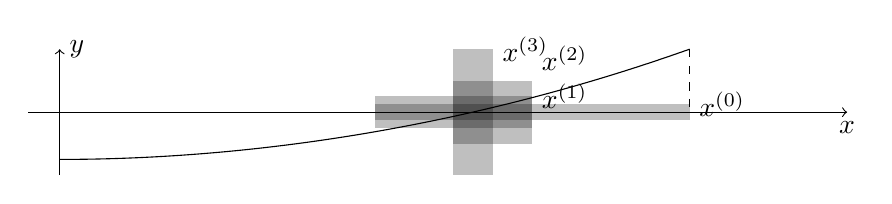
\begin{tikzpicture}[scale=2,fill opacity=0.25,text opacity=1]
\draw[->] (-0.2,0) -- (5,0) node [below] {$x$};
\draw[->] (0,-0.4) -- (0,0.4) node [right] {$y$};
\draw (0,-0.3) parabola (4,0.4);
\draw[dashed] (4,0.4) -- (4,0);
\fill[black] (2,-0.05) rectangle (4,0.05) node [right] {$x^{(0)}$};
\fill[black] (2,-0.1) rectangle (3,0.1) node [right] {$x^{(1)}$};
\fill[black] (2.5,-0.2) rectangle (3,0.2) node [above right] {$x^{(2)}$};
\fill[black] (2.5,-0.4) rectangle (2.75,0.4) node [right] {$x^{(3)}$};
\end{tikzpicture}
\caption{二分法示意(重叠的灰色格子即不断缩窄的区间套)}\label{7-f1}
\end{figure}


\entry \key{简单迭代法}:构造非线性方程 $f(x)=0$ 的同解变形 $x=\vphi(x)$,例如
\[ x = x - f(x),\quad x=\sqrt{x^2-kf(x)} \]
等,再构造对应迭代格式为
\begin{equation}
x_{k+1}=\vphi(x_k).
\end{equation}
若 $\{x_k\}$ 收敛到 $x^\ast$,且 $\vphi(x)$ 也在 $x^\ast$ 处连续,则对以上方程左右取极限即得 $x^\ast=\vphi(x^\ast)$,说明该迭代法可以逼近方程之解。

\entry \key{Newton 法}:设非线性方程 $f(x)=0$ 之解为 $x^\ast$,即 $x^\ast = 0$,将其
在 $x_k$ 处展开可得
\begin{equation}\label{7-e2}
f(x_k)+f'(x_k)(x^\ast-x_k)+\cdots = 0
\end{equation}
舍去二阶项,有 $f(x_k)+f'(x_k)(x^\ast-x_k)\approx0$,进而可变换得到
\[x^\ast\approx x_k-\frac{f(x_k)}{f'(x_k)}\]
改写其为一个迭代格式即得
\begin{equation}\label{7-e1}
x_{k+1} = x_k-\frac{f(x_k)}{f'(x_k)}
\end{equation}
可验证该方程确为 $f(x)=0$ 的同解变形,故该迭代格式收敛时必能得到方程之解。(根据 Newton 法的几何意义,其又被称为\key{切线法}。)

\entry \key{改进 Newton 法}:在上面的展开式 \eqref{7-e2} 中保留到二次项,可解得:
\[ x^\ast\approx x_k+\frac{-f'(x_k)\pm\sqrt{f'(x_k)^2-2f(x_k)f''(x_k)}}{f''(x_k)} \]
分母中的正负号不定,故可写出两种迭代格式:
\begin{gather}
\tilde{x}_{k+1}=x_k-\frac{f'(x_k)+\sgn(f'(x_k))\sqrt{f'(x_k)^2-2f(x_k)f''(x_k)}
}{f''(x_k)},\\
\overline{x}_{k+1}=x_k-\frac{2f(x_k)}{f'(x_k)+\sgn(f'(x_k))\sqrt{f'(x_k)^2-2f(x_k)
f''(x_k)}}.
\end{gather}
选取 $\tilde{x}_{k+1}$ 与 $\overline{x}_{k+1}$ 中距离 $x_k$ 更近者,作为下一步迭代
时的 $x_{k+1}$ 即可。

\entry \key{简化 Newton 法}:若 $f'(x)$ 难以计算,可将迭代格式 (\ref{7-e1}) 改写为
\begin{equation}
x_{k+1}=x_k-\frac{f(x_k)}{f'(x_0)}
\end{equation}
即始终采用\emph{初值点处导数}近似表示 $f'(x_k)$。

\entry \key{弦割法}
\footnote{弦割法的提出已有相当历史,西安交大 120 周年校庆时提出的「风云两甲子,\emph{弦割}三世纪」即是为纪念其悠久的历史而作。}
:将迭代格式 (\ref{7-e1}) 中的导数 $f'(x_k)$ 用两点数值微分公式代替,可
得到:
\begin{itemize}
    \item 若用 $x_k$ 与 $x_{k-1}$ 作为迭代格式中的两点,则得
    \begin{equation}
    x_{k+1} = x_k-\frac{f(x_k)}{\frac{f(x_k)-f(x_{k-1})}{x_k-x_{k-1}}} =
    x_k-\frac{f(x_k)(x_k-x_{k-1})}{f(x_k)-f(x_{k-1})}
    \end{equation}
    此即\key{两点弦割法}。
    \item 若用 $x_k$ 与 $x_0$ 作为迭代格式中的两点,则得
    \begin{equation}
    x_{k+1} = x_k-\frac{f(x_k)}{\frac{f(x_k)-f(x_0)}{x_k-x_0}} =
    x_k-\frac{f(x_k)(x_k-x_0)}{f(x_k)-f(x_0)}
    \end{equation}
    此即\key{单点弦割法}。
\end{itemize}

\entry 弦割法需要给定\emph{两步}初值 $x_0$ 与 $x_1$ 才能进行,它们通常由其他方法获得。

\entry 切线法与弦割法的几何意义:如图 \ref{7-f2} 所示。
\begin{figure}[htbp]
\small\centering
\begin{tikzpicture}[xscale=2,yscale=4]
\draw[->] (0,0) -- (1.2,0) node [above] {$x$};
\draw[->] (0,-0.2) -- (0,1) node [right] {$y$};
\draw (0,-0.15) parabola (1.2,1) node [left] {$f(x)$};
\draw[dashed] (1,0.65) -- (1,0) node [below] {$x^{(0)}$};
\draw[red] (1.2,0.95) -- (1,0.65) -- (0.567, 0) node [below,black] {$x^{(1)}$};
\draw[dashed] (0.567,0) -- (0.567,0.108);
\draw[blue] (0.801,0.324) -- (0.567,0.108) -- (0.45,0);
\draw[dashed] (0.45,0) -- (0.45,0.3) node [above] {$x^{(2)}$};
\node at (0.6,-0.2) {Newton 法};
\end{tikzpicture}\hfil
\begin{tikzpicture}[xscale=2,yscale=4]
\draw[->] (0,0) -- (1.2,0) node [above] {$x$};
\draw[->] (0,-0.2) -- (0,1) node [right] {$y$};
\draw (0,-0.15) parabola (1.2,1) node [left] {$f(x)$};
\draw[dashed] (1,0.65) -- (1,0) node [below] {$x^{(0)}$};
\draw[red] (1.2,0.95) -- (1,0.65) -- (0.567, 0) node [below,black] {$x^{(1)}$};
\draw[dashed] (0.567,0) -- (0.567,0.108);
\draw[blue] (0.644,0.216) -- (0.49,0);
\draw[dashed] (0.49,0) -- (0.49,0.3) node [above] {$x^{(2)}$};
\node at (0.6,-0.2) {简化 Newton 法};
\end{tikzpicture}\hfil
\begin{tikzpicture}[xscale=2,yscale=4]
\draw[->] (0,0) -- (1.2,0) node [above] {$x$};
\draw[->] (0,-0.2) -- (0,1) node [right] {$y$};
\draw (0,-0.15) parabola (1.2,1) node [left] {$f(x)$};
\draw[dashed] (1.1,0) -- (1.1,0.807) node [left] {$x^{(0)}$};
\draw[dashed] (0.679,0) -- (0.679,0.22) node [right] {$x^{(1)}$};
\draw[red] (1.2,0.95) -- (1,0.67) -- (0.679,0.22) -- (0.521,0) node [below,black] {$x^{(2)}$};
\draw[dashed] (0.521,0) -- (0.521,0.068);
\draw[blue] (0.986,0.524) -- (0.679,0.22) -- (0.521,0.068) -- (0.456,0);
\draw[dashed] (0.456,0) -- (0.456,0.2) node [above] {$x^{(3)}$};
\node at (0.6,-0.2) {两点弦割法};
\end{tikzpicture}\hfil
\begin{tikzpicture}[xscale=2,yscale=4]
\draw[->] (0,0) -- (1.2,0) node [above] {$x$};
\draw[->] (0,-0.2) -- (0,1) node [right] {$y$};
\draw (0,-0.15) parabola (1.2,1) node [left] {$f(x)$};
\draw[dashed] (1.1,0) -- (1.1,0.807) node [left] {$x^{(0)}$};
\draw[dashed] (0.679,0) -- (0.679,0.22) node [right] {$x^{(1)}$};
\draw[red] (1.2,0.95) -- (1,0.67) -- (0.679,0.22) -- (0.521,0) node [below,black] {$x^{(2)}$};
\draw[dashed] (0.521,0) -- (0.521,0.068);
\draw[blue] (1.2,0.934) -- (0.521,0.068) -- (0.468,0);
\draw[dashed] (0.468,0) -- (0.468,0.2) node [above] {$x^{(3)}$};
\node at (0.6,-0.2) {单点弦割法};
\end{tikzpicture}
\caption{迭代解法的几何意义}\label{7-f2}
\end{figure}

\section{迭代法的收敛理论}
\entry 迭代法的两种\setkey{收敛性}{迭代法收敛性}:设非线性方程 $f(x)=0$ 在 $[a,b]$ 上有解 $x^\ast$,取定迭代格式 $x_{k+1}=\vphi(x_k)$ 与初值 $x_0$。若
\begin{itemize}\tl
    \item 存在 $x^\ast$ 的一个小邻域,使得只要 $x_0$ 在此邻域中就能保证 $\{x_k\}$ 收
    敛\footnote{根据迭代格式的意义,当 $\{x_k\}$ 收敛时其必收敛于 $x^\ast$。}
    ,则称迭代格式\key{局部收敛};
    \item 对任意的 $x_0\in[a,b]$,都有 $\{x_k\}$ 收敛,则称迭代格式\key{全局收敛}。
\end{itemize}

\trm \key{全局收敛定理}(压缩映射原理):设 $\vphi(x)\in C[a,b]$,且满足:
\begin{enumerate}\tl
    \item $x\in[a,b]$ 时,$\vphi(x)\in[a,b]$;
    \item 存在 $L\in[0,1)$,使得对任意的 $x\in[a,b]$都有
    \begin{equation}
    |\vphi'(x)|\leq L<1.
    \end{equation}
\end{enumerate}
则由 $\vphi(x)$ 所构造的 $x_{k+1}=\vphi(x_k)$ 将是一个在 $[a,b]$ 上全局收敛的迭代
数列,且其满足以下\emph{误差估计式}:
\begin{gather}
|x^\ast-x_k|\leq\frac{L^k}{1-L}|x_1-x_0|,\quad\text{(先验估计)}\\
|x^\ast-x_k|\leq\frac1{1-L}|x_{k+1}-x_k|.\quad\text{(事后估计)}
\end{gather}

\entry 以上定理的结果,仅是全局收敛的\emph{充分条件},而非\emph{必要条件}。

\trm \key{局部收敛定理}:设方程 $f(x)=0$ 有解 $x^\ast$,利用其同解变形构造了一个迭代格式
$x_{k+1}=\vphi(x_k)$。若存在 $x^\ast$ 的某邻域 $[x^\ast-\delta,x^\ast+\delta]$ 使
\[ |\vphi'(x)|\leq L<1 \]
则迭代格式 $x_{k+1}=\vphi(x_k)$ 在该邻域上\emph{局部收敛}。

\trm Newton 迭代法的\emph{局部收敛定理}:设非线性方程 $f(x)=0$ 有解 $x^\ast$,在 $x^\ast$
附近 $f(x)$ 二阶连续可微,$f'(x^\ast)\neq0$,则 Newton 迭代格式 (\ref{7-e1}) 在 
$x^\ast$ 的充分小邻域内局部收敛。(或:当初值 $x_0$ \emph{充分靠近} $x^\ast$ 时,Newton
迭代法收敛。)

\trm Newton 迭代法的\emph{全局收敛定理}:设非线性方程 $f(x)=0$ 在 $[a,b]$ 上有解 $x^\ast$,
且 $f(x)$ 在 $[a,b]$ 上二阶连续可微。则 Newton 迭代格式 (\ref{7-e1}) 在 $[a,b]$ 上
全局收敛的充分条件是:
\begin{enumerate}\tl
    \item $f(a)\cdot f(b)<0$;
    \item 对任意的$x\in[a,b]$,$f'(x)\neq0$;
    \item $f''(x)$ 在 $[a,b]$ 上不变号;
    \item 初值 $x_0$ 满足 $f(x_0)f''(x_0)>0$。
\end{enumerate}

\trm 弦割法\emph{局部收敛}的条件与 Newton 法类似,只要 $x_0,x_1$ 两步初值充分靠近 $x^\ast$。

\trm 弦割法\emph{全局收敛定理}:在 Newton 法的所有条件之基础上,还应附加满足 $f(x_1)f''(x_1)
>0$。

\define \key{收敛阶}:设 $\{x_k\}$ 按某种迭代格式收敛于方程的解 $x^\ast$,若存在常数 $p\geq1$
与 $c>0$ 使条件
\begin{equation}
\lim_{k\to\infty}\frac{|x^\ast-x_{k+1}|}{|x^\ast-x_k|^p}=c\neq0
\end{equation}
成立,则称 $\{x_k\}$ 以 $p$ 阶收敛到方程之解。称 $c$ 为\emph{渐进误差常数}。

\entry $p=1$时,称为\key{线性收敛},否则称为\key{超线性收敛}。

\trm (整数)\key{收敛阶定理}:设 $\vphi(x)$ 在不动点上 $x^\ast$ 的邻域内有连续的 $p$ 阶
导数,则由 $x_{n+1}=\vphi(x_k)$ 生成的 $\{x_k\}$ 以 $p$ 阶收敛的充要条件是:
\[\vphi'(x^\ast)=\vphi''(x^\ast)=\cdots=\vphi^{(p-1)}(x^\ast)=0,\,\vphi^{(p)}
(x^\ast)\neq0.\]

\entry 常见迭代格式的\emph{收敛阶}:
\begin{itemize}\tl
    \item \emph{简单迭代法}:当 $0<|\vphi'(x^\ast)|<1$时\emph{线性收敛}。
    \item \emph{Newton 法}:当 $f'(x)\neq0$时\emph{二阶收敛}。
    \item \emph{两点弦割法}:满足收敛条件时具有 $p=\frac{1+\sqrt5}2\approx1.618$ 的收敛阶,\emph{超线性收敛}。
    \item \emph{单点弦割法}:满足收敛条件时\emph{线性收敛}。 
\end{itemize}

\entry \key{加速收敛方法}:促使原来收敛较慢的算法更快收敛,或使原来发散的迭代格式变为收敛。

\entry \key{松弛因子加速法}:对迭代格式 $x=\vphi(x)$,在方程左右减去一带\emph{松弛因子} $\omega$
的项 $\omega x$,得
\[ x-\omega x=\vphi(x)-\omega x \]
进而可得新的收敛格式
\begin{equation}
x=\frac{\vphi(x)-\omega x}{1-\omega}=\psi(x)
\end{equation}
为检查该迭代格式的收敛性,可以对其求导得
\[ \psi'(x)=\frac1{1-\omega}(\vphi'(x)-\omega) \]
若代入 $\omega=\vphi'(x^\ast)$,则在 $x^\ast$ 附近时 $|\psi(x^\ast)|$ 相当小,由此即
可保证 $|\psi'(x)|\leq L<1$ 的条件成立(将发散的迭代格式改进为收敛的),并提高收敛速率。

\entry \key{Aitken 加速法}:略
\footnote{参见李乃成、梅立泉《数值分析》第228页「艾特肯加速法」,该加速方法是在假设迭代格式线性收敛的情况下作出的。}。
